\chapter{Using the Flash Subsystem API}

In this chapter we explain how to use the NAND subsystem API to describe and simulate a NAND flash based storage subsystem.

\section{Basics}

\subsection{The Address object}
To address a specific object (page, block, plane, etc.) of the simulated flash subsystem, the Address object is used. Addressing is essential of course when sending commands, but also for other functions of the simulator such as gathering statistics on a given subset of the subsystem after a simulation. In the flash subsystem, an address is from a theoretical point of view a tuple of 6 elements represented as follows: 

\begin{center}
$(a, b, c, d, e, f)$
\end{center}

The members of this tuple are:
\begin{itemize}
  \item $a$ is the channel index in the whole flash subsystem ;
  \item $b$ is the chip index in the channel ;
  \item $c$ is the die index in the chip ;
  \item $d$ is the plane index in the die ;
  \item $e$ is the block index in the plane ;
  \item $f$ is the page index in the block.
\end{itemize}

For example, consider a flash system with 2 channels, 4 chips per channel, 2 dies per chip, 2 planes per die, 2048 blocks per plane and 64 pages per block. If we want to address, for instance during a legacy read operation, the seventh page (page 6) in the 100th block (block 99) of the second plane (plane 1) of the first die (die 0) of the third chip (chip 2) of the first channel (channel 0) of such a subsystem, the tuple locating this exact page will be: $(0,2,0,1,99,6)$.

Note that for certain operations, the lowest levels members of the address are not significant. For example, if one want to erase the block containing the page of our previous example, the page member of the address is insignificant because we target the whole block and not a particular page in this block. Therefore, any number can be passed for the page member of the address, OpenFlash will not perform any address range check on that member.

At the code level, an address object is simply created with the Address class:

\begin{lstlisting}
Address a1(0,2,0,1,99,6);
Address *a2 = new Address(0,2,0,1,99,6);
/* do some things with a1 and *a2 */
delete a2;
\end{lstlisting}

After instantiating, one can retrieve the members of the address using getters functions, and modify them with setters:

\begin{lstlisting}
int channel = a1.getChannel();  // Channel is 0
a1.setDie(1);                   // Die member of a1 is now equal to 1
\end{lstlisting}

Comparison functions (\verb+==+ and \verb+!=+) are also available:

\begin{lstlisting}
Address a3(1,2,0,1,99,6);
Address a4(0,1,0,1,1501,60);

bool res = (a3 == a4);    // res is false
bool res = (a3 != a4);    // res is true
\end{lstlisting}

For more information on the Address object, see the technical documentation here: \href{http://stockage.univ-brest.fr/~polivier/sample_doc/classAddress.html}{\textit{http://stockage.univ-brest.fr/~polivier/sample\_doc/classAddress.html}}

\subsection{The Error Manager}
That entity is used to centralize the error management in OpenFlash. Each simulation program realized with OpenFlash must have one instance of the error manager. It is declared as \verb+extern+ in one of OpenFlash headers (common.h), and must be defined as a global variable in the main file of the simulation program. The way the error manager is defined is explained hereafter.

The error manager is called from various points in the OpenFlash sources. When an error or a problem arises during a simulation, the error manager is called an the simulation may be stopped according to the gravity of the error. OpenFlash error manager defines two types of problems:

\begin{enumerate}
  \item \emph{Warnings} are not fatal to the functioning of the simulation, and the simulation may continue after a warning. The role of the warning is to indicate that something unanticipated may have happen. It will in practice take the form of a warning message on the standard / error output ;
  \item \emph{Errors} are serious and indicate that something went wrong during the simulation. In practice the simulation should not continue after an error.
\end{enumerate}

Example of errors are writing in a page already containing data, out-of-range addressing during commands sending, etc. An example of warning is the fact that a page write operation does not occur sequentially in a block. Note that for now, most of the problems that may occur in OpenFlash are \emph{errors}.

At the current stage, the error manager takes two parameters:

\begin{enumerate}
  \item The fact that a simulation should stop on a \emph{warning} ;
  \item The fact that a simulation should stop on an \emph{error}.
\end{enumerate}

It is recommended to set the error manager not to stop the simulation on a warning, and to stop the simulation on an error. Setting that a simulation should \emph{not} stop on an error is reserved for unit testing / debugging, and should never be set this way during a real simulation.

In practice, the simulator \emph{stops} the simulation by executing the following instruction: \verb+assert(0)+. This allows keeping the program context in some debuggers such as gdb, for debugging purposes.

As stated earlier, the error manager object is declared as '\verb+extern ErrorManager em;+' in one of OpenFlash headers. It must be defined at global scope in the main file of the simulation program, as follows:

\begin{lstlisting}
ErrorManager em(false, true, true);
\end{lstlisting}

The constructor of the ErrorManager object takes 3 parameters which are all booleans:

\begin{itemize}
  \item The first parameter indicates if the simulation should be stopped on an error ;
  \item The second parameter indicates if the simulation should be stopped on a warning ;
  \item The last parameter indicates if a warning should be throwed when a non sequential write occurs within a block.
\end{itemize}

The error manager will be used by the flash subsystem layer of OpenFlash, but the user may also use it in his own code. To throw a warning or an error, proceed as follows:

\begin{lstlisting}
em.warning("This is a warning");
em.error("This is an error");
\end{lstlisting}

As the error manager is declared at global scope, one should be able to call it from anywhere in the program. The error / warning message will be printed on the error output and the program will continue or be stopped according to the parameters of the error manager.

For more information concerning the ErrorManager class see the related technical documentation at the following URL:
\href{http://stockage.univ-brest.fr/~polivier/sample_doc/classErrorManager.html}{\textit{http://stockage.univ-brest.fr/~polivier/sample\_doc/classErrorManager.html}}.

\subsection{Basic simulation template \& compiling}

Defining and executing a simulation require to create one or several C++ files, one of these files containing a \verb+main+ function. These files must include the OpenFlash sources which present some dependencies, in particular with the libconfig library. The libconfig library is used by OpenFlash to provide configuration file support, its use is explained in a following section of this document.

Here we present how to build a simulation from a single main C++ file. The file must be present at the root of OpenFlash source (with the others OpenFlash source files). This main file must include the \verb+FlashSystem.hpp+ header, a \verb+main+ function, and the definition of the error manager as explained earlier. A basic template for a simulation program should then be as follows:

\begin{lstlisting}
#include <iostream>   // some standard includes ...
#include <cstdlib>    // ... for practical reasons

#include "FlashSystem.hpp"    // OpenFlash flash subsystem header

ErrorManager em(false, true, true);   // error manager

int main(int argc, char **argv)       // Main function
{
  return EXIT_SUCCESS;
}
\end{lstlisting} 

Consider this file is named MySimulation.cpp. To be able to compile it edit the OpenFlash Makefile as follows:

\begin{lstlisting}[language=sh, firstnumber=15]
# Executable targets (cpp with main functions):
UNITTESTS=UnitTests.cpp
EXAMPLE=Example.cpp
MYSIMULATION=MySimulation.cpp       # Add this line ...
# Full list
FULLSRCS=$(SRCS) $(UNITTESTS) $(MYSIMULATION) # ... and the variable here
FULLHEADERS=$(SRCS:.cpp=.hpp) $(UNITTESTS:.cpp=.hpp)

# Then add at the end of the following line a target with the name of your choice:
all: libconfig UnitTest++ UnitTests Example MySimulation
\end{lstlisting}
%%$

Then add the following target:

\begin{lstlisting}[language=sh, firstnumber=50]
# My simulation:
MySimulation: $(SRCS:.cpp=.o) $(MYSIMULATION:.cpp=.o)
	$(CXX) $(CXXFLAGS) $(INCLUDES) $^ -o $@ $(LDFLAGS)
\end{lstlisting}

Typing \verb+make+ in a shell at the root of OpenFlash sources should then trigger the compiling of your (empty) simulation file, and all its dependencies. You should observe the creation of a \verb+MySimulation+ executable at the end of the process. Note that for now OpenFlash makefile performs static compiling with the libraries. We are aware that static compiling is not considered as a good programming practice. However, the current goal is to distribute OpenFlash in a self sufficient archive, and we want OpenFlash not to be subject to bugs due to library code changes.

\section{Defining the structure and functions of the simulated flash subsystem}

The simulated flash subsystem is represented by the C++ class FlashSystem, which is the core of the OpenFlash flash subsystem layer. You can find plenty of information about the FlashSystem class in this document. This information can be completed by the technical documentation concerning the FlashSystem class. It can be found at the following URL: \href{http://stockage.univ-brest.fr/~polivier/sample_doc/classFlashSystem.html}{\textit{http://stockage.univ-brest.fr/~polivier/sample\_doc/classFlashSystem.html}}.

The structural parameters for the simulated flash subsystem are defined when instantiating the FlashSystem object. They are:

\begin{enumerate}
  \item The number of pages per block ;
  \item The number of blocks per plane ;
  \item The number of planes per die ;
  \item The number of dies per chip ;
  \item The number of chips per channel ;
  \item The total number of channels in the flash subsystem.
\end{enumerate}

These values are passed as parameters, in reverse order, to the FlashSystem constructor. The following example creates a FlashSystem object with 2 channels, 4 chips per channels, 2 dies per chip, 2 planes per die, 2048 blocks per plane and 64 pages per block:

\begin{lstlisting}
FlashSystem f1(2,4,2,2,2048,64);
\end{lstlisting}

To describe a FlashSystem with just one chip having the same structure as above:

\begin{lstlisting}
FlashSystem f2(1,1,2,2,2048,64);
\end{lstlisting}

Once the FlashSystem  object is instantiated, one can get the structural parameters using "getters" functions, such as:

\begin{lstlisting}
int pagesPerBlock = f1.getPagesPerBlockNum();   // Number of pages per block, here it is 64
int channels = f1.getChannelNum();  // Number of channels, here 2

int totalPageNum = f1.getPageNum();   // Total number of pages in the FlashSystem, here it is 2*4*2*2*2048*64 = 4194304
\end{lstlisting}

When a FlashSystem object is instantiated, it supports by default all the flash commands (described in the previous chapter). One can deactivate the support of some commands as follows:

\begin{lstlisting}
// Indicate that the flash subsystem does not support die interleaved multi plane commands:

f1.setSupportedCommands(DIE_INTERLEAVED_MULTI_PLANE_READ, false);
f1.setSupportedCommands(DIE_INTERLEAVED_MULTI_PLANE_WRITE, false);
f1.setSupportedCommands(DIE_INTERLEAVED_MULTI_PLANE_ERASE, false);
f1.setSupportedCommands(DIE_INTERLEAVED_MULTI_PLANE_CACHE_READ, false);
f1.setSupportedCommands(DIE_INTERLEAVED_MULTI_PLANE_CACHE_WRITE, false);

// One can also reactivate the support for some commands:
f1.setSupportedCommands(DIE_INTERLEAVED_MULTI_PLANE_CACHE_WRITE, true);
\end{lstlisting}

The name of the command in upper case is define by the OpenFlash flash command model which will be depicted in details in the next section. Deactivating the support of some commands will result in an error thrown if one of these command is issued to the simulated system during the simulation.

\section{Sending commands to the flash subsystem}
There are two ways to send a command to the flash subsystem during the simulation:

\begin{description}
  \item[Method 1] By using one of the member function of the FlashSystem object, according to the command one want to send. For example, the FlashSystem class provides a FlashSystem::readPage() method to perform a legacy page read operation. There is one function for each of the supported commands.
  \item[Method 2] By using the FlashSystem::receiveCommand() method, taking a \emph{FlashCommand} object as parameter. This object describes the command sent to the flash subsystem.
\end{description}

In fact, the method 1 above is just an encapsulation which internally creates a \emph{FlashCommand} object according to the operation and call the \\\verb+FlashSystem::receiveCommand()+ method. The FlashCommand class implements the OpenFlash flash command model and is used to describe a given flash operation ready to be sent to the flash subsystem. The OpenFlash flash command model is detailed in the next sections.

All commands except multi chips and multi channels commands can be sent to the FlashSystem object through method 1. It is easier because one does not have to bother with instantiating a FlashCommand object. Nevertheless, multi chips and multi channels commands consists both in a set commands sent on multiple chips / multi ple channels. These commands can be of \emph{any} type\footnote{Note that a multi chip command cannot contain a multi channel / multi chip command, and that a multi channel command cannot contain itself a multi channel command}. Therefore OpenFlash uses arrays of generic types to describe the sets of commands constituting multi chips / channels commands. This generic type is the FlashCommand type.

\colorbox{red}{TODO Explain the flash command model.}

In the following sections we explain with examples how to send all types of commands using method 1 (member functions). Next, after having depicted the OpenFlash flash command model, when explain how to use method 2 (\\\verb+FlashSystem::receiveCommand()+ function).

\subsection{Method 1 : FlashSystem member functions}

In this section we describe all the \verb+FlashSystem+ object member functions used to send flash commands through method 1. We give for each function its prototype, explanations on the parameters and return values. We also list all the error that may lead the command to fail. Note that although all these member functions return -1 in case of error, if the error manager is configured to stop the program in case of error the program will be killed before the function can return.

\subsubsection{Sending legacy operations}

Legacy operations are page read, page write, and block erase operations. Sending such operations through method 1 consist in calling the following member functions:

\begin{itemize}
  \item \verb+FlashSystem::readPage(Address a)+
  \begin{itemize}
    \item Parameter \verb+a+ is the address of the page to read ;
    \item This function returns 0 on success, 1 if the page read is empty (which can be considered as a success or a failure according to the situation), and -1 on error. For now the only error that can occur when sending a legacy read command is the fact that one of the members of the address is out of range in the flash system: for example targeting a page in the block 4000 in a flash system with 2048 blocks per plane.
  \end{itemize}
  
  \item \verb+FlashSystem::writePage(Address a)+
  \begin{itemize}
    \item Parameter \verb+a+ is the address of the page to read ;
    \item This function returns 0 on success, -1 on error. An error can be due to various situations:
    \begin{itemize}
      \item Out of range addressing ;
      \item The targeted page already contains data.
    \end{itemize}
  \end{itemize}
  
  \item \verb+FlashSystem::eraseBlock(Address a)+
  \begin{itemize}
    \item The parameter \verb+a+ is the address of the block to erase (the page member of this address is not significant) ;
    \item This function returns 0 on success and -1 on error. An error is due to out of range addressing.
  \end{itemize}
\end{itemize}

Below are some examples of sending legacy operations through method 1.
\begin{lstlisting}
int res;
FlashSystem f(2,4,2,2,2048,64);           /* declare simulated system */

res = f.readPage(Address(1,3,0,0,33,60));                /* read a page */
res = f.writePage(Address(1,3,0,0,0,0));                 /* write a page */
res = f.eraseBlock(Address(0,2,1,1,0,0));                /* erase a block */
\end{lstlisting}

\subsubsection{Sending cache and copy back operations}

These operation are sent through the following methods:

\begin{itemize}
  \item \verb+FlashSystem::cacheRead(Address startPage, int nbPagesToRead)+
  \begin{itemize}
    \item \verb+startPage+ is an address targeting the first page to read ;
    \item \verb+nbPagesToRead+ is the number of pages to read sequentially, starting from \verb+startPage+ ;
    \item This function returns 0 on success, a positive integer equal to the number of empty pages read if any. It returns -1 on error. An error can be due to several situations:
    \begin{itemize}
      \item Out of range addressing for \verb+firstPage+ ;
      \item The set of pages to read crosses the containing block boundaries ;
      \item \verb+nbPagesToRead+ is equal to 0.
    \end{itemize}
  \end{itemize}
  
  \item \verb+FlashSystem::cacheWrite(Address startPage, int nbPagesToWrite)+
  \begin{itemize}
    \item This function works the same way as \verb+cacheRead+. The return value is a bit different: it is 0 on success and -1 on error. Errors can be due to the same situations as with \verb+cacheRead+. Another cause of error for \verb+cacheWrite+ is the fact that one of the written pages already contains data.
  \end{itemize}
  
  \item \verb+FlashSystem::copyBack(Address source, Address target)+
  \begin{itemize}
    \item \verb+source+ and \verb+target+ are the addresses of the source page (read) and the target page (written) of the copy back operation.
    \item This function returns 0 on success, -1 on error. An error is due to the following situations:
    \begin{itemize}
      \item Out of range addressing for \verb+source+ and / or \verb+target+ ;
      \item \verb+source+ and \verb+target+ are not in the same plane ;
      \item \verb+source+ and \verb+target+ have the same address ;
      \item The page index in the containing block for \verb+source+ and \verb+target+ are not both odd or both even.
    \end{itemize}
  \end{itemize}
\end{itemize}

Below is an example of cache read and write operations, as well as a copy back operation example.

\begin{lstlisting}
int res;
FlashSystem f(2,4,2,2,2048,64);           /* declare simulated system */

/* read the entire block 0 :*/
res = f.cacheRead(Address(0,0,0,0,0,0), 64);

/* write the first half of block 3 :*/
res = f.cacheWrite(Address(0,0,0,0,3,0), 32);

/* Copy back from the first page of block 0 to the page 32 of block 3 :*/
res = f.copyBack(Address(0,0,0,0,0,0), Address(0,0,0,0,3,32));
\end{lstlisting}

\subsubsection{Sending multi plane operations}
As presented earlier, multi plane operation have one constraint saying that the read / write / erase operation must be performed on \emph{all} the planes of the same die. Moreover all these sub-operations must be performed at the same location within the targeted planes. Therefore, to describe a multi-plane operation in OpenFlash, one need only to specify the address of \emph{one} page (for multi plane read \& write) or \emph{one} block (multi plane erase) and the tool will automatically apply this operation on all the planes of the die containing the targeted page / block.

Sending multi plane operation is done through the following functions:

\begin{itemize}
  \item \verb+FlashSystem::multiPlaneRead(Address a)+
  \begin{itemize}
    \item \verb+a+ is the address of one page to read, the multi plane operation will automatically be applied on all the planes of the targeted die ;
    \item This function return 0 on success, a positive integer representing the number of empty pages read if any, and -1 on error. An error may be due to out of range addressing.
  \end{itemize}
  
  \item \verb+FlashSystem::multiPlaneWrite(Address a)+
  \begin{itemize}
    \item Works in a similar way to the \verb+multiPlaneRead+ function ;
    \item Returns 0 on success, -1 on error. An error may be due to out of range addressing, or to the fact that one of the written pages already contains data.
  \end{itemize}
  
  \item \verb+FlashSystem::multiPlaneErase(Address a)+
  \begin{itemize}
    \item Returns 0 on success, -1 on error (out of range addressing).
  \end{itemize}
\end{itemize}

Below are some examples of multi plane read, write and erase operations.

\begin{lstlisting}
int res;
FlashSystem f(2,4,2,2,2048,64);           /* declare simulated system */

/* multi plane read in (1,3,1,0,124,12) and (1,3,1,1,124,12) */
res = f.multiPlaneRead(Address(1,3,1,1,124,12));

/* multi plane write in (0,2,0,0,12,4) and (0,2,0,1,12,4) */
res = f.multiPlaneWrite(Address(0,2,0,0,12,4));

/* multi plane erase in (0,0,0,0,122,X) and (0,0,0,1,122,X) */
res = f.multiPlaneErase(Address(0,0,0,0,122,0));
\end{lstlisting}

Note that a warning is thrown when sending a multi plane operation in a flash subsystem with only one plane per die.

\subsubsection{Sending die interleaved operations}
Die interleaved operations constraints are lighter than multi plane ones:
\begin{enumerate}
  \item Die interleaved operations can concern only a subset of all the dies in a chip ;
  \item Targeted pages / blocks of one die interleaved operation may be in different locations within the concerned die.
\end{enumerate}

Therefore, to describe a die interleaved operation in OpenFlash, one must use arrays. OpenFlash makes an intensive use of C++ standard \verb+vector+ type. The parameters of OpenFlash functions used to send die interleaved operations takes vectors of addresses as parameters. Each member of the vector is one page to read / write, or one block to erase. Each member must be in a different die of the same chip.

Sending die interleaved operations is done through the use of the following functions:

\begin{itemize}
  \item \verb+FlashSystem::dieInterleavedRead(vector<Address> addresses)+
  \begin{itemize}
    \item \verb+addresses+ is an array of Address objects, each one targeting a page to read in a different die of the same chip ;
    \item This function returns 0 on success, a positive integer equal to the number of empty pages read if any, and -1 on error. An error may be due to the following situations:
    \begin{itemize}
      \item Out of range addressing for one of the members of \verb+addresses+ ;
      \item The members of \verb+addresses+ are not in different dies of the same chip.
    \end{itemize}
  \end{itemize}
  
  \item \verb+FlashSystem::dieInterleavedWrite(vector<Address> addresses)+
  \begin{itemize}
    \item Works the same way as the die interleaved read function ;
    \item Returns 0 on success, -1 on error. Errors may occur in the same situations as with the die interleaved read function. An error is also returned when one of the written pages already contains data.
  \end{itemize}
  
  \item \verb+FlashSystem::dieInterleavedErase(vector<Address> addresses)+
  \begin{itemize}
    \item Works the same way as the die interleaved read / write functions ;
    \item Return 0 on success, -1 on error. An error is due to out of range addressing.
  \end{itemize}
\end{itemize}

Below are some examples of die interleaved read / write / erase operations.

\begin{lstlisting}
int res;
FlashSystem f(2,4,2,2,2048,64);           /* declare simulated system */

/* die interleaved read on (1,2,0,1,339,12) and (1,2,1,1,339,12) :*/
vector<Address> addresses_read;
addresses_read.push_back(Address(1,2,0,1,339,12)); 
addresses_read.push_back(Address(1,2,1,1,339,12));
res = f.dieInterleavedRead(addresses_read);

/* die interleaved write on (0,1,0,1,145,60) and (0,1,1,1,229,12) :*/
vector<Address> addresses_write;
addresses_write.push_back(Address(0,1,0,1,145,60)); 
addresses_write.push_back(Address(0,1,1,1,229,12));
res = f.dieInterleavedWrite(addresses_write);

/* die interleaved erase on (1,0,0,0,222,X) and (1,0,1,1,444,X) :*/
vector<Address> addresses_erase;
addresses_erase.push_back(Address(1,0,0,0,222,0)); 
addresses_erase.push_back(Address(1,0,1,1,444,X));
res = f.dieInterleavedErase(addresses_erase);
\end{lstlisting}

Note that a warning is thrown when sending a die interleaved operation in a flash subsystem containing only one die per chip.

\subsubsection{Sending multi plane cache \& copy back operations}
Multi plane cache operations are described with one start page and a number of page to read / write. The described cache operation is automatically applied on all the planes of the targeted die.

Multi plane copy back operations works the same way: they are described with only one couple of addresses for the source and target pages of the operation. The copy back is the performed automatically in all the planes of the targeted die.

The functions used to send multi plane cache and copy back operations are:

\begin{itemize}
  \item \verb+FlashSystem::multiPlaneCacheRead(Address startPage, int nbPagesToRead)+
  \begin{itemize}
    \item \verb+startPage+ is the address of the first page to read in \emph{one} of the targeted planes ;
    \item \verb+nbPagesToRead+ is the number of pages to read in each copy back of the multi plane copy back operation
    \item The operation will automatically be performed in all the planes of the die targeted by \verb+startPage+ ;
    \item This operation returns 0 on success, a positive integer equal to the number of empty pages read if any, and -1 on error. An error can occur in various situations:
    \begin{itemize}
      \item \verb+startPage+ is out of range ;
      \item \verb+startPage+ + \verb+nbPagesToRead+ crosses the containg block boundaries ;
      \item \verb+nbPagesToRead+ is 0.
    \end{itemize}
  \end{itemize}
  
  \item \verb+FlashSystem::multiPlaneCacheWrite(Address firstPage, int nbPagesToWrite)+
  \begin{itemize}
    \item Works in a similar way as the multi plane cache read function ;
    \item Returns 0 on success, -1 on error. In addition to the errrors previously evocated in the multi plane cache read function, the multi plane cache write function may generate an error if one of the pages written is already containing data.
  \end{itemize}
  
  \item \verb+FlashSystem::multiPlaneCopyBack(Address source, Address target)+
  \begin{itemize}
    \item \verb+source+ and \verb+target+ are the source and target page of a copy back oepration in \emph{one} plane. The same copy back operation will automatically be performed in all the planes of the target die.
    \item Returns 0 on success, -1 on error. An error can signify that:
    \begin{itemize}
      \item \verb+source+ or \verb+target+ is out of range ;
      \item Page index within their blocks for \verb+source+ and \verb+taret+ are not both odd or both even.
      \item \verb+source+ and \verb+target+ are requal or not in the same plane.
    \end{itemize}
    
  \end{itemize}
\end{itemize}

Below are some examples of multi plane copy back and cache oeprations.

\begin{lstlisting}
int res;
FlashSystem f(2,4,2,2,2048,64);           /* declare simulated system */

/* Multi plane cache read on the entirety of the first block of planes
 * (0,2,1,0,X,X) and (0,2,1,1,X,X) */
res = f.multiPlaneCacheRead(Address(0,2,1,0,0,0), 64);

/* Multi plane cache write on the first half of the first block of 
 * planes (0,1,0,0,X,X) and (0,1,0,1,X,X) */
res = f.multiPlaneCacheWrite(Address(0,1,0,0,0,0), 32);

/* Multi plane copy back from (1,1,0,0,122,12) to (1,1,0,0,444,14) and
 * from (1,1,0,1,122,12) to (1,1,0,0,444,14) */
res = f.multiPlaneCopyBack(Address(1,1,0,0,122,12), Address(1,1,0,0,444,14));
\end{lstlisting}

Note that sending these operation may throw a warning when the simulated flash subsystem only contains one plane per die.

\subsubsection{Sending die interleaved cache \& copy back operations}
Die interleaved cache operation must be described by 2 arrays. The first array (named \verb+firstPages+) is a list of addresses for the first pages to read / write. The second array (names \verb+nbPagesToRead+ / \verb+write+) is a list of integer representing the number of pages to read or write. Therefore, each couple \verb+firstPages+[i], \verb+nbPagesToRead/Write+[i] represent a cache operation that will be applied in one die. Each address in array A must the targets a different die in the same chip. \verb+firstPages+[i] + \verb+nbPageToRead/Write+[i] must not cross block boundaries. Each member of the couple must target the same die. There must not be 2 couples which target the same die.

Die interleaved copy back operations are also described by 2 arrays: \verb+sources+ and \verb+targets+. Each couple \verb+sources[i]+, \verb+targets[i]+ represent a copy back operation to perform in a die. Each member of the couple must target the same die. There must not be 2 couples which target the same die.

OpenFlash functions used to send die interleaved cache and copy back commands are the followings:

\begin{itemize}
  \item \verb+FlashSystem::dieInterleavedCacheRead(vector<Address> startPages,+\\\verb+vector<int> nbPagesToRead)+
  \begin{itemize}
    \item Each cache read operation composing the die interleaved cache read operation is represented by a couple \verb+startPages[i]+, \verb+nbPagesToRead[i]+. Each cache read operation must satisfy the related constraints ;
    \item Returns 0 on success, a positive integer equal to the number of empty pages read if any, -1 on error. An error can signify that:
    \begin{itemize}
      \item The two vector parameters do not have the same sizes ;
      \item Targeted addresses are not in the same chip, or each cache operation is not in different dies of the same chip ;
      \item Out of range addressing.
    \end{itemize}
  \end{itemize}
  
  \item \verb+FlashSystem::dieInterleavedCacheWrite(vector<Address> startPages,+\\\verb+vector<int> nbPagesToWrite)+
  \begin{itemize}
    \item Works in a similar way than the die interleaved cache read function ;
    \item Return 0 on success, -1 on error. In addition to the error causes evocated for the die interleaved read function, the die interleaved write function fails if one of the written pages already contain data.
  \end{itemize}
  
  \item \verb+FlashSystem::dieInterleavedCopyBack(vector<Address> sources,+\\\verb+vector<Address> targets)+
  \begin{itemize}
    \item Each copy back operation composing the die interleaved copy back operation is represented by a couple \verb+sources[i]+, \verb+targets[i]+. Each couple must satisfy the copy back constraints (in particular the source and target member of each couple must be in the same plane).
    \item Returns 0 on success, -1 on error. Errors can be:
    \begin{itemize}
      \item The two vector parameters do not have the same size ;
      \item One of the copy back operations have source and targets that are not in the same plane ;
      \item One of the copy back operations have source and targets index within conataining block that are not both odd or both even ;
      \item Each couple \verb+sources[i]+, \verb+targets[i]+ is not loacted in a different die of the same chip.
    \end{itemize}
  \end{itemize}
\end{itemize}

Below are some examples of die interleaved cache and copy back operations.

\begin{lstlisting}
int res;
FlashSystem f(2,4,2,2,2048,64);           /* declare simulated system */

/* die interleaved cache read for the first half of block (0,1,0,1,2044,X)
 * and the second half of block (0,1,1,0,1054,X) */
vector<Address> startPagesRead;
vector<int> nbPagesToRead;
startPagesRead.push_back(Address(0,1,0,1,2044,0)); nbPagesToRead.push_back(32);
startPagesRead.push_back(Address(0,1,1,0,1054,32)); nbPagesToRead.push_back(32);
res = f.dieInterleavedCacheRead(startPagesRead, nbPagesToRead);

/* die interleaved cache write the whole block (1,0,0,0,154,X) and the 
 * second half of block (1,0,1,1,12,X) */
vector<Address> startPagesWrite;
vector<int> nbPagesToWrite;
startPagesWrite.push_back(Address(1,0,0,0,154,0)); nbPagesToWrite.push_back(64);
startPagesWrite.push_back(Address(1,0,1,1,12,32)); nbPagesToWrite.push_back(32);
res = f.dieInterleavedCacheWrite(startPagesWrite, nbPagesToWrite);

/* Die interleaved copy back from (0,3,0,1,144,12) to (0,3,0,1,120,60)
 * and from (0,3,1,0,12,51) to (0,3,1,0,255,53) */
vector<Address> sources; vector<Address> targets;
sources.push_back(Address(0,3,0,1,144,12));
targets.push_back(Address(0,3,0,1,120,60));
sources.push_back(Address(0,3,1,0,12,51));
targets.push_back(Address(0,3,1,0,255,53));
res = f.dieInterleavedCopyBack(sources, targets);
\end{lstlisting}

\subsubsection{Sending die interleaved multi plane operations}
Die interleaved multi plane read operations are characterized by one array. Each member of this array is a multi plane read operation composing the whole die interleaved multi plane read operation. Each member must then target a different die in the same chip. The multi plane read operation will be applied automatically in all the planes of the targetted die.

The die interleaved multi plane write / erase operation work in a similar way than the die interleaved multi plane read. These operation are sent with the following functions:

\begin{itemize}
  \item \verb+FlashSystem::DieInterleavedMultiPlaneRead+\\\verb+(vector<Address> addresses)+
  \begin{itemize}
    \item Takes as parameter a vector of addresses, each one in a different die of the same chip. The multi plane read operation represented by each member of that vector will automatically applied in all the planes of the targetted die.
    \item Returns 0 on success, a positive interger equal to the number of empty pages read if any, -1 on error. An arror may be due to the following situations:
    \begin{itemize}
      \item Out of range addressing ;
      \item Each member of \verb+addresses+ does not target a different die of the same chip ;
      \item The size of \verb+addresses+ is superior to the number of dies per chip.
      \item 
    \end{itemize} 
  \end{itemize}
  
  \item \verb+FlashSystem::DieInterleavedMultiPlaneWrite+\\\verb+(vector<Address> addresses)+
  \begin{itemize}
    \item Works the same way as the die interleaved multi plane read function.
    \item Returns 0 on success, -1 on error. In addition to the errors mentionned for the die interleaved multi plane read function, the write funtion fails when one of the written pages already contains data.
  \end{itemize}
  
  \item \verb+FlashSystem::DieInterleavedMultiPlaneErase+\\\verb+(vector<Address> addresses)+
  \begin{itemize}
    \item Works the same way as the die interleaved multi plane read / write functions.
  \end{itemize}
\end{itemize}

Below are some examples of die interleaved multi plane read / write / erase functions.

\begin{lstlisting}
int res;
FlashSystem f(2,4,2,2,2048,64);           /* declare simulated system */

/* die interleaved multi plane read targetting the following addresses :
 * (1,2,0,0,144,62) ; (1,2,0,1,144,62) ; (1,2,1,0,12,11) ; (1,2,1,1,12,11)
 */
vector<Address> addr_read;
addr_read.push_back(Address(1,2,0,0,144,62));
addr_read.push_back(Address(1,2,1,0,12,11));
res = f.dieInterleavedMultiPlaneRead(addr_read);

/* die interleaved multi plane write targetting the following addresses :
 * (0,1,0,0,12,0) ; (0,1,0,1,12,0) ; (0,1,1,0,4,0) ; (0,1,1,1,4,0)
 */
vector<Address> addr_write;
addr_write.push_back(Address(0,1,0,0,12,0));
addr_write.push_back(Address(0,1,1,0,4,0));
res = f.dieInterleavedMultiPlaneWrite(addr_write);

/* die interleaved multi plane erase targetting the following addresses :
 * (0,3,0,0,255,X) ; (0,3,0,1,255,X) ; (0,3,1,0,4,X) ; (0,3,1,1,4,X)
 */
vector<Address> addr_erase;
addr_erase.push_back(Address(0,3,0,0,255,0));
addr_erase.push_back(Address(0,3,1,0,4,X));
res = f.dieInterleavedMultiPlaneErase(addr_erase);
\end{lstlisting}

The die interleaved multi plane cache read and write operation are characterized by two arrays. Consider the die interleaved multi plane cache read operation. The first array \verb+startPages[]+ is a list of first pages to read. The second array \verb+nbPagesToRead+ is a list of number of pages to read. Each couple \verb+startPage[i]+, \verb+nbPagesToRead[i]+ describe then a multi plane cache read operation (see section concerning multi plane cache operations). The entirety of the couples describe the die interleaved multi plane cache read operation.

Die interleaved multi plane cache write works the same way. To send such types of operations, the following functions are used:

\begin{itemize}
  \item \verb+FlashSystem::dieInterleavedMultiPlaneCacheRead+\\\verb+(vector<Address> firstPages, vector<int> nbPagesToRead)+
  \begin{itemize}
    \item \verb+firstPages[i]+ and \verb+nbPagesToRead[i]+ describe the multi plane cache read operations launched in the dies ;
    \item This function returns 0 on success, a positive integer equal to the number of empty pages read if any, and -1 on error. An error may signify that:
    \begin{itemize}
      \item The size of \verb+firstPages+ and the size of \verb+nbPagesToRead+ are different, or superior to the number of dies per chip ;
      \item Out of range addressing ;
      \item One couple \verb+startPages[i]+, \verb+nbPagesToRead[i]+ do not satisfy multi plane cache read constraints ;
      \item Each multi plane cache read operation do not target a different die int the same chip.
    \end{itemize}
  \end{itemize}
  
  \item \verb+FlashSystem::dieInterleavedMultiPlaneCacheWrite+\\\verb+(vector<Address> firstPages, vector<int> nbPagesToWrite)+
  \begin{itemize}
    \item This function works in a similar way than the die interleaved multi plane cache read function, with the addition that it may fail when one of the written page already contains data.
  \end{itemize}
\end{itemize}

Below are some examples of die interleaved multi plane cache read / write operations.

\begin{lstlisting}
int res;
FlashSystem f(2,4,2,2,2048,64);           /* declare simulated system */

/* Die interleaved multi plane cache read on the entire block 0 of 
 * (1,2,0,0,X,X), (1,2,0,1,X,X) and the entire block 1 of 
 * (1,2,1,0,X,X), (1,2,1,1,X,X) */
vector<Address> startPagesR;
vector<int> nbPagesToRead;
startPagesR.push_back(Address(1,2,0,0,0,0));
nbPagesToRead.push_back(64);
startPagesR.push_back(Address(1,2,1,0,0,0));
nbPagesToRead.push_back(64);
res = f.dieInterleavedMultiPlaneCacheRead(startPagesR, nbPagesToRead);

/* Die interleaved multi plane cache read on the first half of block 12 of 
 * (1,2,0,0,X,X), (1,2,0,1,X,X) and the entire block 1 of 
 * (1,2,1,0,X,X), (1,2,1,1,X,X) */
vector<Address> startPagesW;
vector<int> nbPagesToWrite;
startPagesW.push_back(Address(1,2,0,0,0,0));
nbPagesToWrite.push_back(32);
startPagesW.push_back(Address(1,2,1,0,0,0));
nbPagesToWrite.push_back(64);
res = f.dieInterleavedMultiPlaneCacheWrite(startPagesW, nbPagesToWrite);
\end{lstlisting}

Note that all the die interleaved multi plane functions throw a warning when launched on a simulated subsystem with only one plane per die or one die per chip.

\subsubsection{Sending multi chips / channels commands}

As explained earlier, sending multi chips or multi channels commands involves instantiating a \emph{FlashCommand} object.

\subsection{Method 2 : FlashSystem::receiveCommand}

\begin{figure}
  \center
  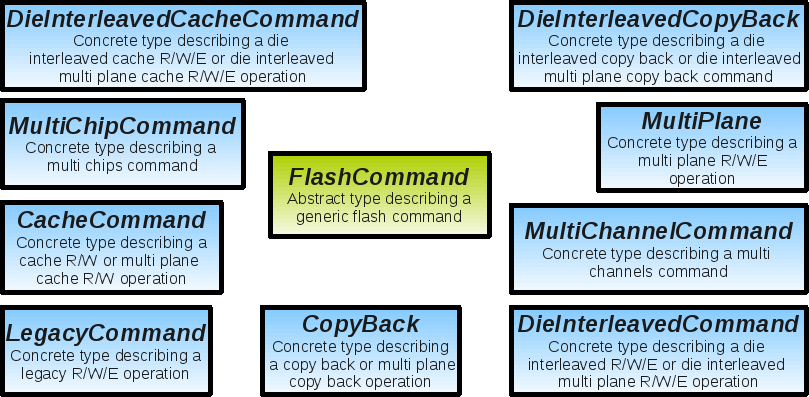
\includegraphics[width=0.9\textwidth]{Includes/FlashCommandModel.png}
  \caption{The different types (C++ classes) used by OpenFlash to describe a flash command}
  \label{fig:flashcommandmodel}
\end{figure}

\subsubsection{OpenFlash flash command model}






\section{Describing the performance and power consumption behavior}

\colorbox{red}{TODO.}

\section{Using the configuration file}
OpenFlash uses \emph{libconfig}\footnote{\href{http://www.hyperrealm.com/libconfig/}{\textit{http://www.hyperrealm.com/libconfig/}}} to provide support for a configuration file. It is a text file containing blocks of key values pairs that can be used to define the parameters of the whole simulated systems, and the parameters for the simulation itself (for example error management parameters).

\subsection{The Param object}

\section{Gathering simulation results}

\colorbox{red}{TODO.}

